\section{Christoffer}
\subsection{Overview}
% \begin{frame}{Christoffer}
% \begin{itemize}
%   \only<1->{\item This}
%   \only<2->{\item is}
%   \only<3->{\item a}
%   \only<4>{\item test}
% \end{itemize}
% \end{frame}


%================================ Intro ============================
\begin{frame}{Christoffer: Overview}
\begin{itemize}
  \item Technical Details
  		\begin{itemize}
  			\item How was REST implemented
  			\item The impact of the REST implementation
  			\item Asynchronous requests and the problems they cause
  			\item Request chaining
  			\item Activity controllers
		\end{itemize}
  \item Showcase the Launcher
\end{itemize}
\end{frame}

%================================ Technical Details ============================
\subsection{Technical Details}
\begin{frame}[fragile]{How was REST implemented}
\only<1>{
\begin{itemize}
  \item Replace old database models usage
  \begin{itemize}
  \item DB\_lib to REST models
\end{itemize}
  \item First version of REST vs current version
\end{itemize}

}

\begin{onlyenv}<2>
\begin{itemize}
  \item Replace old database models usage
    \begin{itemize}
  \item DB\_lib to REST models
\end{itemize}
\end{itemize}
\begin{center}
\begin{minipage}[H]{0.9\linewidth}
\begin{lstlisting}
public LoadApplicationTask(final Context context, final Profile currentUser,
final Profile guardian, final ViewPager appsViewPager, final View.OnClickListener onClickListener)
...
currentUser.getRole() != Profile.Roles.CHILD 
\end{lstlisting} 

to

\begin{lstlisting}    
public LoadApplicationTask(final Context context, final User currentUser,
final User guardian, final ViewPager appsViewPager, final View.OnClickListener onClickListener)
...
!currentUser.hasPermission(PermissionType.User)
\end{lstlisting} 
\end{minipage}
\end{center}
\end{onlyenv}

\begin{onlyenv}<3>
\begin{center}
\begin{minipage}[H]{0.9\linewidth}
\begin{lstlisting}
LoginRequest loginRequest = new LoginRequest(user, new Response.Listener<Integer>() {
	@Override
    public void onResponse(Integer statusCode) {
    	...            
    }            
}, new Response.ErrorListener() {
    @Override
    public void onErrorResponse(VolleyError error) {
    	...
    }
});
queue.add(loginRequest);
\end{lstlisting} 
\begin{lstlisting}    
handler.login(user, new Response.Listener<Integer>() {
	@Override
    public void onResponse(Integer response) {
    	...
    }
}, new Response.ErrorListener() {
    @Override
    public void onErrorResponse(VolleyError error) {
    	... 
    }
});
\end{lstlisting} 
\end{minipage}
\end{center}
\end{onlyenv}
\end{frame}

\begin{frame}[fragile]{REST implementation issues}
\only<1,3>{
\begin{itemize}
  \item Asynchronous issues
  \item Often changes
  \begin{enumerate}
  \item Parameter changes
  	\item Request changes
\end{enumerate}
  \item Mismatch between client lib and server 
  \begin{itemize}
  \item Different class / variable names
\end{itemize}
\end{itemize}
}

\begin{onlyenv}<2>
\begin{center}
\begin{minipage}[H]{0.9\linewidth}
\begin{lstlisting}    
PutRequest<User> userPutRequest = new PutRequest<User>(currentUser, new Response.Listener<User>() {
	@Override
    public void onResponse(User response) {
    	...
    }
}, new Response.ErrorListener() {
    @Override
    public void onErrorResponse(VolleyError error) {
		...
    }
});
queue.add(userPutRequest);
\end{lstlisting} 
\begin{lstlisting}
handler.resourceRequest(currentUser.getSettings(), new Response.Listener<Settings>() {
	@Override
	public void onResponse(Settings response) {
		...	
	}
}, new Response.ErrorListener() {
	@Override
    public void onErrorResponse(VolleyError error) {
    	...
    }
});
\end{lstlisting} 
\end{minipage}
\end{center}
\end{onlyenv}
\end{frame}


\begin{frame}{Asynchronous requests}
\only<1>{
\begin{itemize}
  \item What is the issues?
  \begin{itemize}
  \item Code made for synchronous system 
\end{itemize}
  \item What was the big problem?
  \begin{itemize}
  \item GirafFragment, AndroidFragment
  \item Adapter
\end{itemize}
  \item What caused it and how was it fixed?
  \begin{itemize}
  \item ReloadApplications method call
\end{itemize}
\end{itemize}
}

\begin{onlyenv}<2>
\begin{itemize}
  \item What caused it and how was it fixed?
  \begin{itemize}
  \item ReloadApplications method call
\end{itemize}
\end{itemize}
\begin{center}
\begin{minipage}[H]{0.9\linewidth}
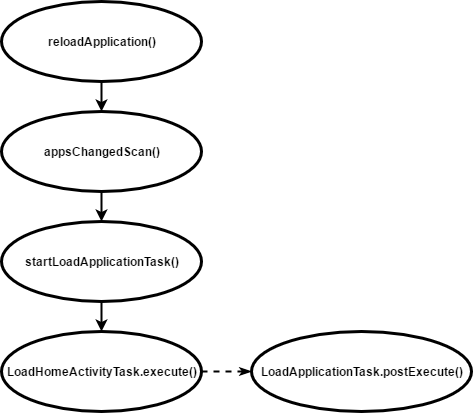
\includegraphics[scale=0.45]{figures/DonDiagram.png} 
\end{minipage}
\end{center}
\end{onlyenv}
\end{frame}

\begin{frame}[fragile]{Request chaining}
\only<1,3>{
\begin{itemize}
  \item Why do we use them?
  \begin{itemize}
  \item Control execution order 
\end{itemize}
  \item How do they look?
  \item Problems with them?
  \begin{itemize}
  \item Many lines of code
  \item Less readable
\end{itemize}
  \item Are they even necessary?
\end{itemize}
}
\begin{onlyenv}<2>
\begin{center}
\begin{minipage}[H]{0.9\linewidth}
\begin{lstlisting}    
handler.get(User.class, new Response.Listener<User>() {
	@Override
    public void onResponse(User response) {
    	... 
    }
}, new Response.ErrorListener() {
	@Override
    public void onErrorResponse(VolleyError error) {
    	handler.login(user, new Response.Listener<Integer>() {
        	@Override
            public void onResponse(Integer response) {
            	handler.get(User.class, new Response.Listener<User>() {
                	@Override
                    public void onResponse(User response) {
                    	... //same code as the other ...
                    }
                }, new Response.ErrorListener() {
                    @Override
                    public void onErrorResponse(VolleyError error) {
						...
                    }
                });
            }
        });
});
\end{lstlisting} 
\end{minipage}
\end{center}
\end{onlyenv}
\end{frame}

\begin{frame}{Activity controllers}
\begin{itemize}
  \item What is their purpose?
  \begin{itemize}
  \item Split UI and logic
\end{itemize}
  \item Why did we do it?
  \begin{itemize}
  \item Make code more readable
  \item Better divide the activities
\end{itemize}
  \item What is missing?
\end{itemize}
\end{frame}

%================================ Showcase program ============================
\subsection{Showcase}
\begin{frame}{Showcase}
\begin{itemize}
  \item Show the Launcher in action
\end{itemize}
\end{frame}
